\chapter*{Introduction}
\section*{Latent variable model}
A latent variable model is a statistical model that relates a set of observable variables (so-called manifest variables) to a set of latent variables.
\\ The motivation behind Latent Variable model is to be able to  capturing complex or conceptual properties of a system that are difficult to quantify or measure directly. For example we can think of a random process that generates millions pixel images of dogs, if we'll want to learn this random process and generate some images it will be a hard task to do because the complex properties of millions of pixels. But if we think of the that random process as follow: first we sampling a breed of a dog (sampling a from the latent variable sphere) and only after that we sampling a picture with the same dog breed' this might lead us to a better model.\\ \\ 
Let's denote $X$ as observed data and $z$ as latent variable of the data that we don't get to observed. \\ In resemble to Bayesian probability  we can look on the distribution of z as the prior, and the distribution of $z|X$ as posterior. We'll assume the data ($X$) will draw independently from $P_{data}$. \\ 
What we usually will want to do is to with the observed data is to find the parameters $\theta$ that maximize the log-likelihood of our data :
\begin{gather*}
\theta = \underset{\theta}{\arg\max} \ log \ p_{\theta}(X)=\underset{\theta}{\arg\max} \sum_{i=1}^{n} log \ p_{\theta}(X^{(i)})=\underset{\theta}{\arg\max} \sum_{i=1}^{n}log \int_z p_{\theta}(X^{(i)}|z)p_{Z}(z)dz
\end{gather*}
In most scenario the upper optimization problem will be hard to compute or even intractable. To over come This problem we can use Monte-Carlo estimator for this integral and just sample from our prior $p_{Z}$ and we'll get the following optimization problem: 
\begin{gather*}
\theta = \underset{\theta}{\arg\max} \sum_{i=1}^{n}log \frac{1}{K} \sum_{k=1}^{K} p_{\theta}(X^{(i)}|z_{k}^{(i)})p_{Z}(z_{k}^{(i)}) \quad , when \ z^{k}\sim p_{Z}
\end{gather*}
The main problem with prior sampling as suggested is that is not very informative. If we look at z as continuous distribution the sampled z's will most likely to cause $p_{\theta}(X^{(i)}|z^{k})$ to be equal to zero, and thus the $\theta$ parameters that we will get from the problem will not be very informative. \\ So we will use Importance sampling and variation inference approach as follow : 
\begin{gather*}
\theta=\underset{\theta}{\arg\max} \sum_{i=1}^{n}log \int_z p_{\theta}(X^{(i)}|z)p_{Z}(z)dz = \underset{\theta}{\arg\max} \sum_{i=1}^{n}log \int_z \frac{q_{\Phi}(z)}{q_{\Phi}(z)}p_{\theta}(X^{(i)}|z)p_{Z}(z)dz= \\ \\ = \underset{\theta}{\arg\max} \sum_{i=1}^{n}log \mathbb{E}_{z \sim q_{\Phi}(z)}[\frac{p_{\theta}(X^{(i)}|z)}{q_{\Phi}(z)}p_{Z}(z)] \approx \underset{\theta}{\arg\max} \sum_{i=1}^{n}log \sum_{k=1}^{K}\frac{p_{\theta}(X^{(i)}|z_{k}^{(i)})}{q_{\Phi}(z_{k}^{(i)})}p_{Z}(z_{k}^{(i)}) \\ \\ , when\ z^{k}\sim q_{\Phi} \ and \ q_{\Phi} \ is \ some \ distribution \ with \ parameters \ \Phi.
\end{gather*}
We can see that a good-informative approximation to $q_{\Phi}(z)$ will be the posterior of z (i.e $z|X^{(i)}$). To achieve a good approximation of $q_{\Phi}(z)$ we'll use KL-diverge and the objective will be: 
\begin{gather*}
\underset{\theta,\Phi}{\arg\max} \sum_{i=1}^{n}log \sum_{k=1}^{K}\frac{p_{\theta}(X^{(i)}|z_{k}^{(i)})}{q_{\Phi}(z_{k}^{(i)})}p_{Z}(z_{k}^{(i)}) - KL(q_{\Phi}(z)||p_{\theta}(z|X))
\end{gather*}
Another derivation to this objection is from Variational Bayesian method, let's find a good approximation to some posterior\\ \\
\begin{gather*}
KL(q(z)||p(z|X))=\mathbb{E}_{z \sim q(z)}[log \ q(z)-log \ p(z|X)] = \\  
= \mathbb{E}_{z \sim q(z)}[log \ q(z) - log \ \frac{p(z,X)}{p(X)}] = \\ 
=(1) \mathbb{E}_{z \sim q(z)}[log \ q(z) - log \ p(z) - log \ p(X|z)] + log \ p(X) \\ 
\end{gather*}
So According to 1 if we want to maximize the log-likelihood we need to maximize : \\ \\
$log \ p(X) = \underbrace{\mathbb{E}_{z \sim q(z)}[-log \ q(z) + log \ p(z) + log \ p(X|z)]}_{ELBO}+KL(q(z)||p(z|X))$ \\ \\
The Evidence lower bound (ELBO) got his name because we can easily conclude that the lower bound for the log-likelihood is : \\ \\
$log \ p(X) = \underbrace{\mathbb{E}_{z \sim q(z)}[-log \ q(z) + log \ p(z) + log \ p(X|z)]}_{ELBO}+KL(q(z)||p(z|X)) \underbrace{\geq}_{KL \geq 0} ELBO $ \\ And indeed we can see that we got the same objective.
\section*{ELBO Maximization}
The problem with the objective that we got ($\mathbb{E}_{z \sim q_{\Phi}(z)}[-log \ q_{\Phi}(z) + log \ p(z) + log \ p_{\theta}(X|z)]+KL(q_{\Phi}(z)||p(z|X))$) is the KL therm, we cant compute this therm because we don't have the posterior function. But we can see that given X, the log-likelihood is not depend on $q_{\Phi}(z)$ so maximize the ELBO therm is equal to minimize the KL-therm so our final optimization problem that we need to solve is: 
\begin{gather*}
\underset{\theta, \Phi}{\arg\max} \mathbb{E}_{z \sim q_{\Phi}(z)}[-log \ q_{\Phi}(z) + log \ p(z) + log \ p_{\theta}(X|z)] \approx \underset{\theta, \Phi}{\arg\max} \sum_{i=1}^{n}log \sum_{k=1}^{K}\frac{p_{\theta}(X^{(i)}|z_{k}^{(i)})}{q_{\Phi}(z_{k}^{(i)})}p_{Z}(z_{k}^{(i)})\\
\end{gather*}
\section*{ELBO Maximization via Neural Network (Variational Auto Encoder and Amortized Inference)}
When trying to solve the ELBO Maximization problem, we first need to choose family of distribution $F$ with parameters $\Phi$ for $q(z)$ (most of the time it will be the normal distribution). Then we wish to to solve : 
\begin{gather*}
\underset{\theta, \Phi}{\arg\max} \ \mathbb{E}_{X\sim data}[\mathbb{E}_{z \sim q_{\Phi}(z)}[-log \ q_{\Phi}(z) + log \ p(z) + log \ p_{\theta}(X|z)]] \approx \\
\approx \underset{\theta, \Phi}{\arg\max} \frac{1}{n}\sum_{i=1}^{n}log \sum_{k=1}^{K}\frac{p_{\theta}(X^{(i)}|z_{k}^{(i)})}{q_{\Phi}(z_{k}^{(i)})}p_{Z}(z_{k}^{(i)})
\end{gather*}
This could be a hard problem to solve,and for every group of $X$ we need to solve it again. But what if instead of optimizing a set of free parameters, we can introduce a parameterized function that maps from observation space $X$ to the parameters of the approximate posterior distribution (As Amortized Inference suggest). In practice, we might introduce a neural network that accepts an observation as input, and outputs the mean and variance parameter for the latent variable associated with that observation. We can then optimize the parameters of this neural network instead of the individual parameters of each observation.  
\begin{figure}[t]
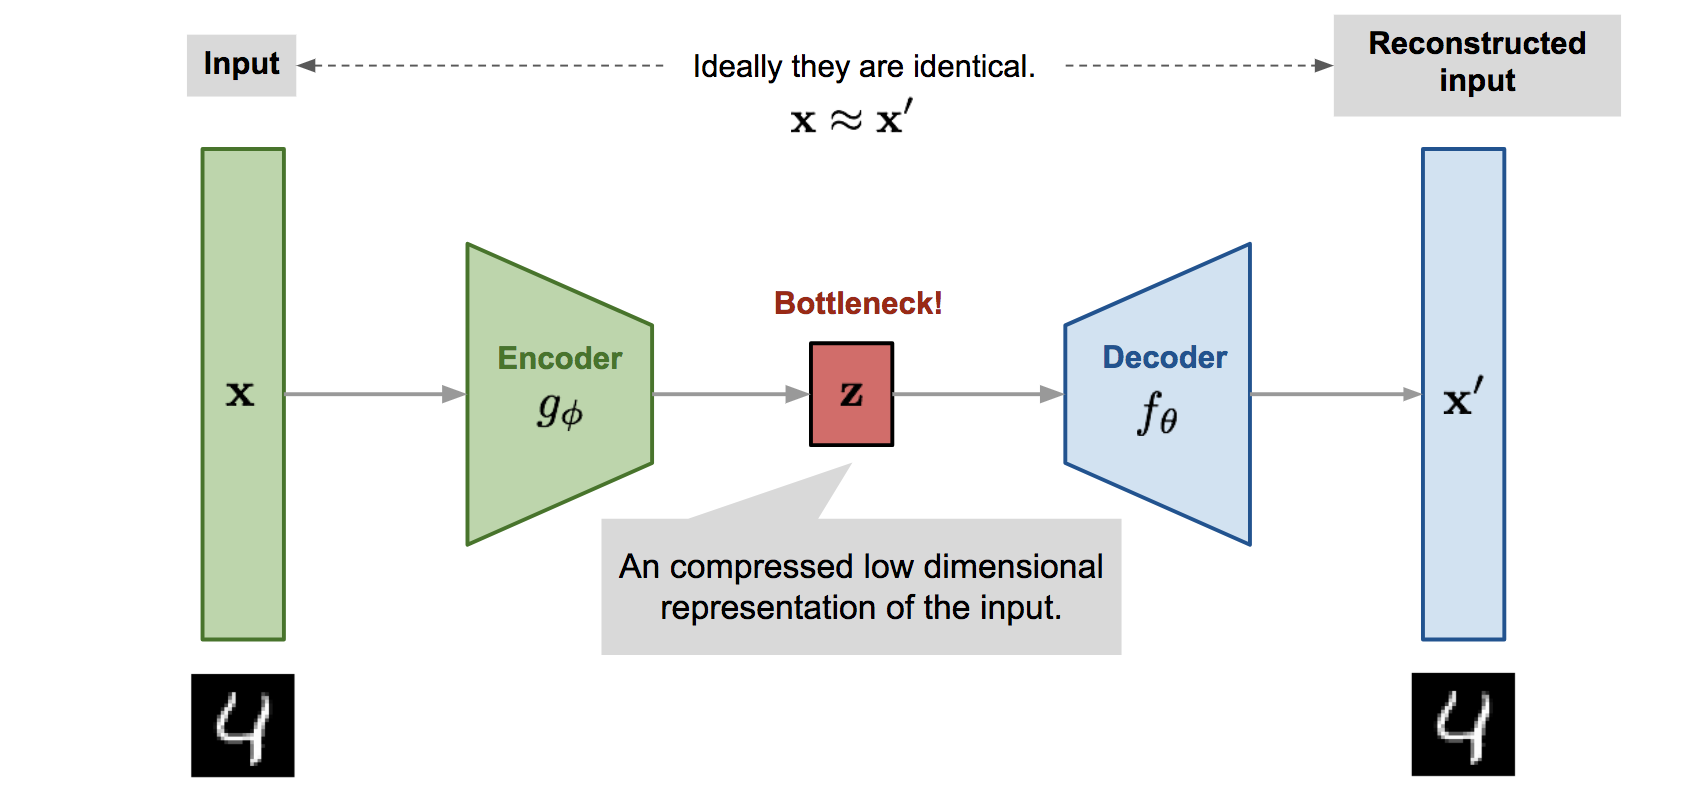
\includegraphics[width=\textwidth]{autoencoder-architecture}
\caption{We can think of this as a encoder (maximize by $\Phi$) and a decoder (maximize by $\theta$)}
\centering
\end{figure}
\\ \\ \\ \\ \\ \\ \\
We can look at the ELBO objective in another interesting way, let rewrite it to another formation :
\begin{gather*}
ELBO=\mathbb{E}_{z \sim q_{\Phi}(z)}[-log \ q_{\Phi}(z) + log \ p(z) + log \ p_{\theta}(X|z)] = \\ \\
= \underbrace{\mathbb{E}_{z \sim q_{\Phi}(z)}[log \ p_{\theta}(X|z)]}_{Reconstruction loss} - \underbrace{KL(q_{\Phi}(z|X)||p(z))}_{Regularization}
\end{gather*}
The Reconstruction therm check if we reconstruct $X$ well : we sample from out estimated posterior $q_{\{Phi}(z)$ and check if that sample is likely to be according to out model (it likely to be if $log \ p_{\theta}(X|z)$ is high. The regularization therm help us to get a regularization to the data we have : the NN model can over fit to the data that we have, i.e find to good approximation to the posterior $q_{\Phi}(z)$. So to prevent that from happens the regularization therm keep the distribution of the posterior simple. \\ \\ \textbf{This is one way to regularize, the paper we about to summarize and check it result is discussing about different way to regularize}.    

\section*{Optimization and representation trick}
We have a optimization problem that we can write like this:
\begin{gather*}
\underset{\theta, \Phi}{\arg\max} \ \mathbb{E}_{z \sim q_{\Phi}(z)}[f(z;\theta)] = \underset{\theta, \Phi}{\arg\max} \int_{z} q_{\Phi}(z)f(z;\theta)dz
\end{gather*}
To solve this problem we'll need to use SGD or GD method, for that we'll need the derivatives. To find the derivatives we need to compute the integral, that might be hard to solve or even intractable. We seen that we can estimate the integral using Monte-Carlo approximation, but this time we have a problem to do that, when we use Monte-Carlo approximation, we can see that the approximation doesn't depend on $\Phi$ anymore, and thus we can't find the derivative w.r.t $\Phi$ \\
To solve that we can rearrange the derivative w.r.t $\Phi$ :
\begin{gather*}
\nabla_{\Phi} (\mathbb{E}_{z \sim q_{\Phi}(z)}[f(z;\theta)]) =  \int_{z} \nabla_{\Phi}(q_{\Phi}(z))f(z;\theta)dz = \int_{z} \frac{q_{\Phi}(z)}{q_{\Phi}(z)}\nabla_{\Phi}(q_{\Phi}(z))f(z;\theta)dz = \\
= \int_{z} q_{\Phi}(z)\nabla_{\Phi}(log \ q_{\Phi}(z))f(z;\theta)dz = \mathbb{E}_{z \sim q_{\Phi}(z)}[\nabla_{\Phi}(log \ q_{\Phi}(z))f(z;\theta)] \approx \\ \approx \frac{1}{K}\sum_{k=1}^{K}\nabla_{\Phi}(log \ q_{\Phi}(z^{(k)})f(z;\theta)
\end{gather*}
This is might look like we solve the problem, but turns out this approximation is very noisy and many samples from $q_{\Phi}$ will be needed. \\
To overcome this issue we can use the representation trick : we can choose $q_{\Phi} \sim N(\mu, \sigma^2)$ and then we can use the normal distribution properties - 
\begin{gather*}
\mathbb{E}_{z \sim q_{\Phi}(z)}[f(z;\theta)] = \mathbb{E}_{\epsilon \sim N(0,I)}[f(\mu_{\Phi} + \sigma_{\Phi}\epsilon;\theta)] \approx \frac{1}{K}\sum_{k=1}^{K}f(\mu_{\Phi} + \sigma_{\Phi}\epsilon^{(k)};\theta), \\ when \ \epsilon^{(k)} \sim N(0,I)
\end{gather*} 
Now to find an estimation for the derivative w.r.t $\Phi$ is easy when we just need to find it (the parameters $\Phi$ are $\mu_{\Phi}, \ \sigma^2_{\Phi}$
\begin{figure}[H]
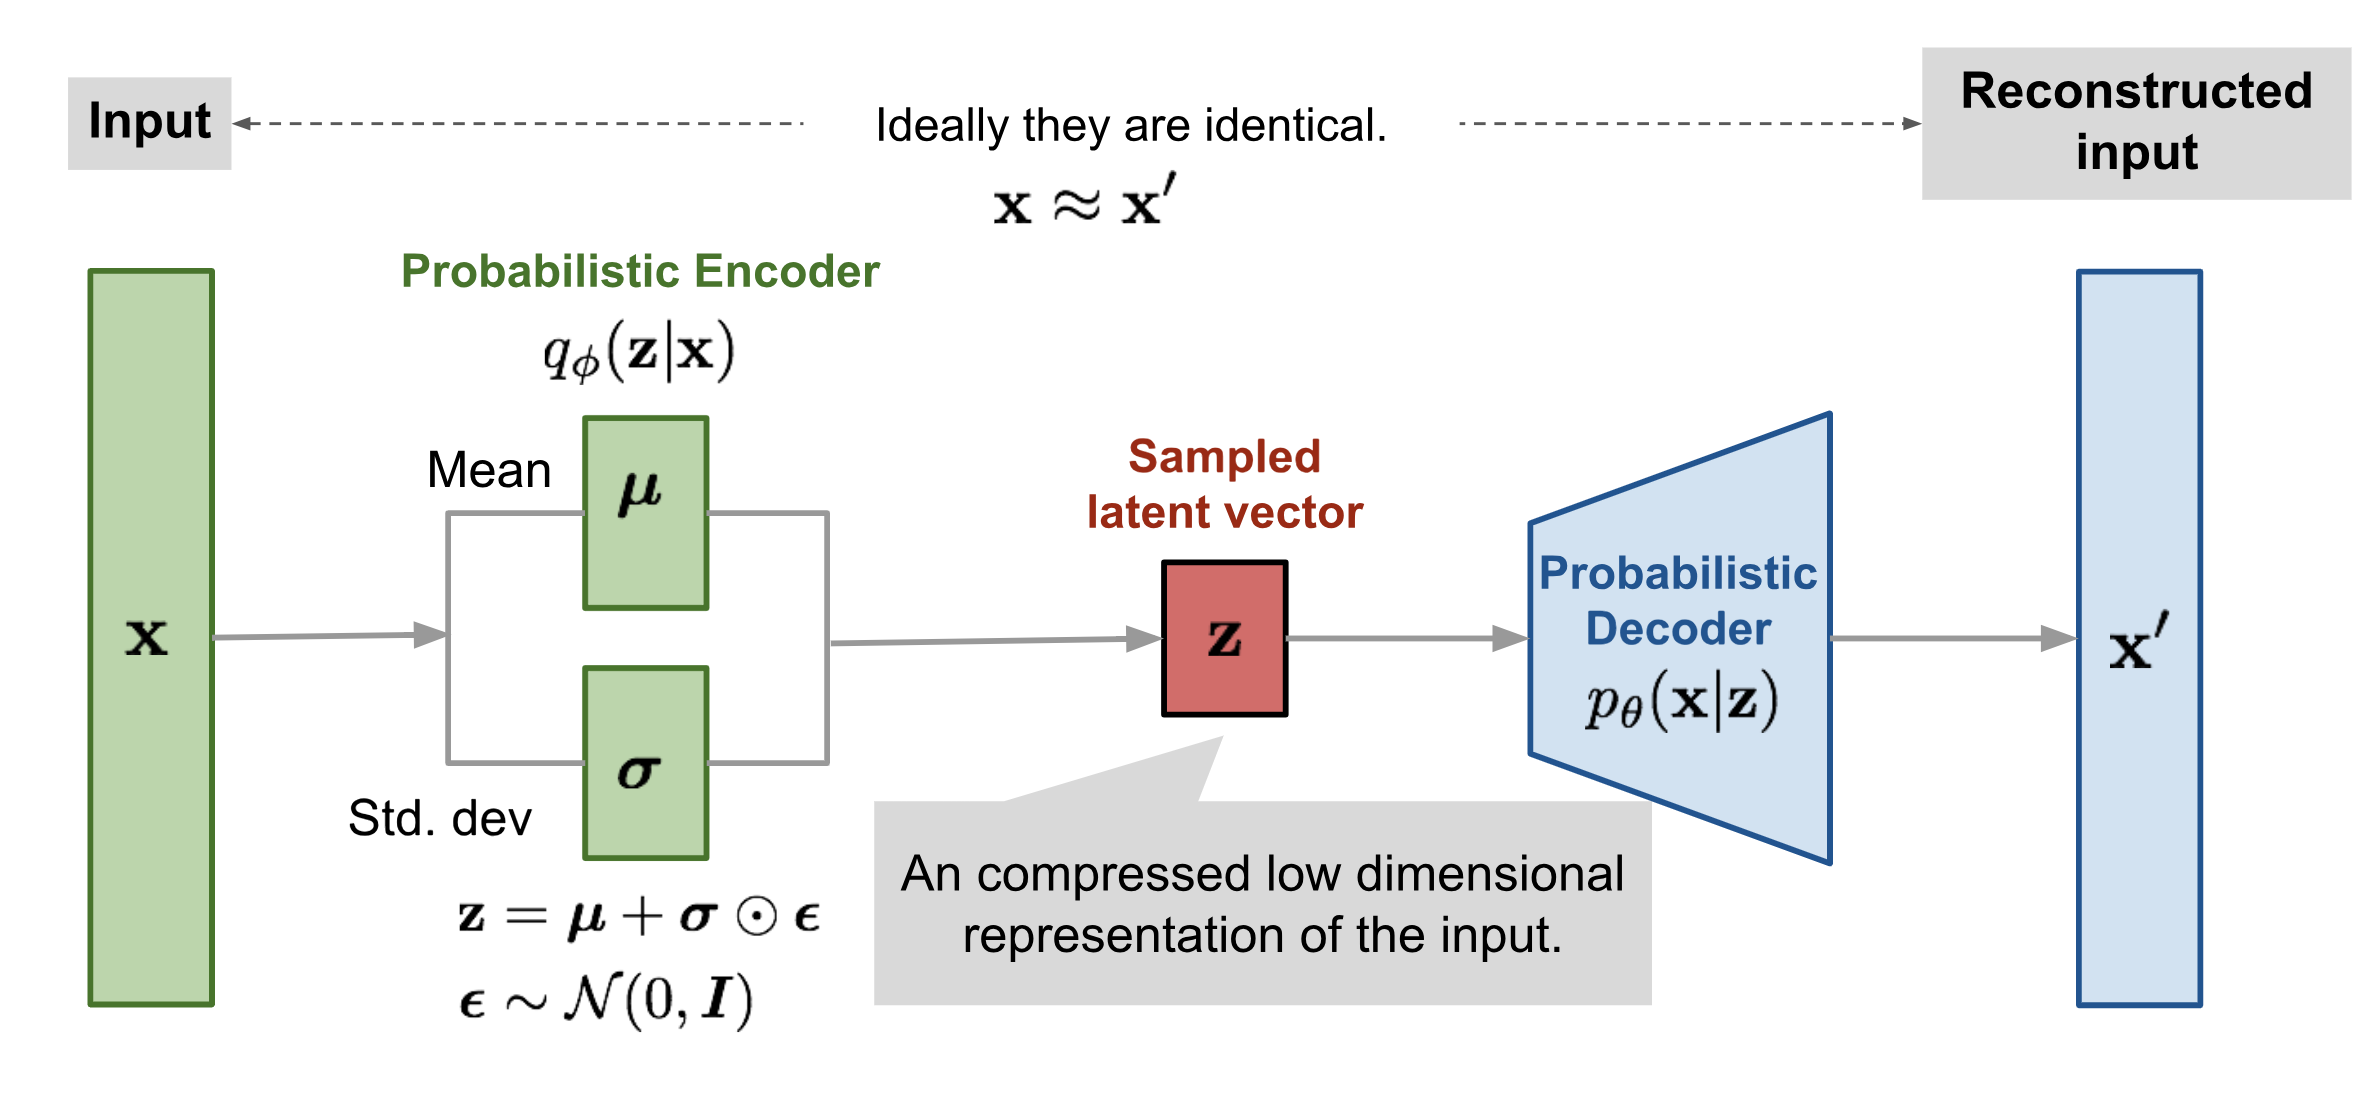
\includegraphics[width=\textwidth]{vae-gaussian}
\caption{To use the representation trick we just need to let $q_{\Phi}\sim N(0,I)$ and find an approximation to the derivative w.r.t $\Phi$ just by sample from the standard Gaussian}
\centering
\end{figure}
